%! Author = sbbfti
%! Date = 10/06/2020


\section{Results}\label{sec:results}

\subsection{Comfort DB overview}\label{subsec:comfort-db-overview}

A total of \var{entries_db_used} entries met the inclusion criteria listed in the Methodology Section.
The distribution of the six input variables used to calculate the PMV indices is depicted in Figure~\ref{fig:dist_input_data}.

\begin{figure}[htb!]
    \centering
    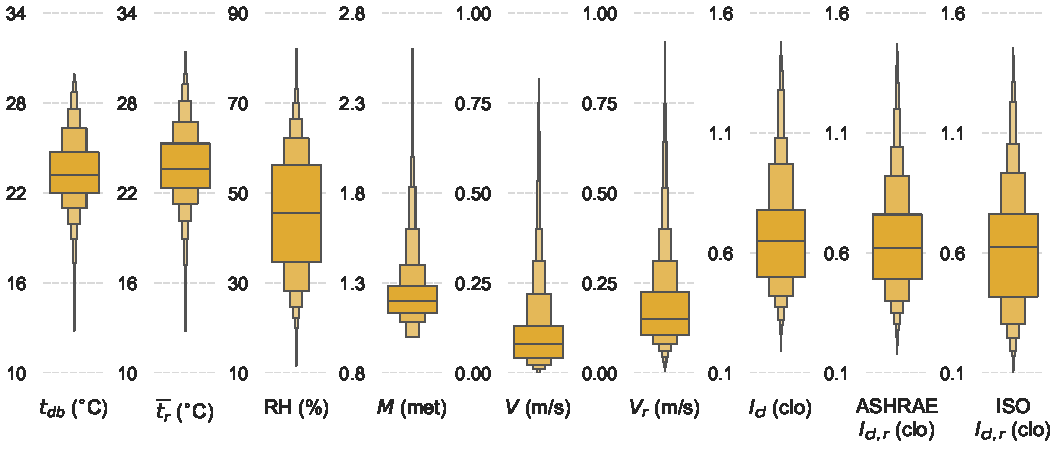
\includegraphics[width=\textwidth]{figures/dist_input_data}
    \caption{Distribution of the input variables used to calculate the \ac{pmv} values.
    The text in blue is showing the the 2.5th, 50th (median), and 97.5th percentiles.
    The data are shown using boxen-plots (letter-value plots).
    They depict the median as the centerline and each successive level outward contains half of the remaining data.}
    \label{fig:dist_input_data}
\end{figure}

Figure~\ref{fig:dist_input_data} also depicts the 2.5th, 50th (median), and 97.5th percentiles for all the input variables.
We were not able to determine the accuracy of the \ac{pmv} formulations for inputs which were lower than the 2.5th and 97.5th percentiles, since we only had a limited number of datapoints beyond those limits.
In natural ventilated buildings \ac{rh} may exceed \var{rh_95_perc_max}, and we could not reliably test the accuracy of the \ac{pmv} formulations for values of \ac{v} higher than \var{v_95_perc_max}.
The latter could be an issue since the \gls{55} permits the use of \ac{v} up to \qty{0.8}{\m\per\sec} even if occupants do not have direct control over the local airspeed.

Figure~\ref{fig:dist_other_data} shows the distribution of the age, height, weight, and running mean outdoor temperature grouped by sex.
Less than half (\num{23300}) of the total entries had information about the participant's sex.
Out of those data were almost equally distributed among male \qty{52}{\percent} and females.
Ages are not normally distributed, the same is true for the running mean outdoor temperature.
About half of the participants (\qty{52}{\percent}) were aged between \num{20} and \num{35} years old, and only \qty{2.5}{\percent} were older than 60.
This limits our analysis to healthy adults, and does not allow us to determine the accuracy of the \ac{pmv} model in predicting thermal sensation for children or older adults.
Approximately \qty{56}{\percent} of the running mean outdoor temperature values where between \qtyrange{10}{25}{\celsius}.
Men were significantly heavier and taller than females.

\begin{figure}[htb!]
    \centering
    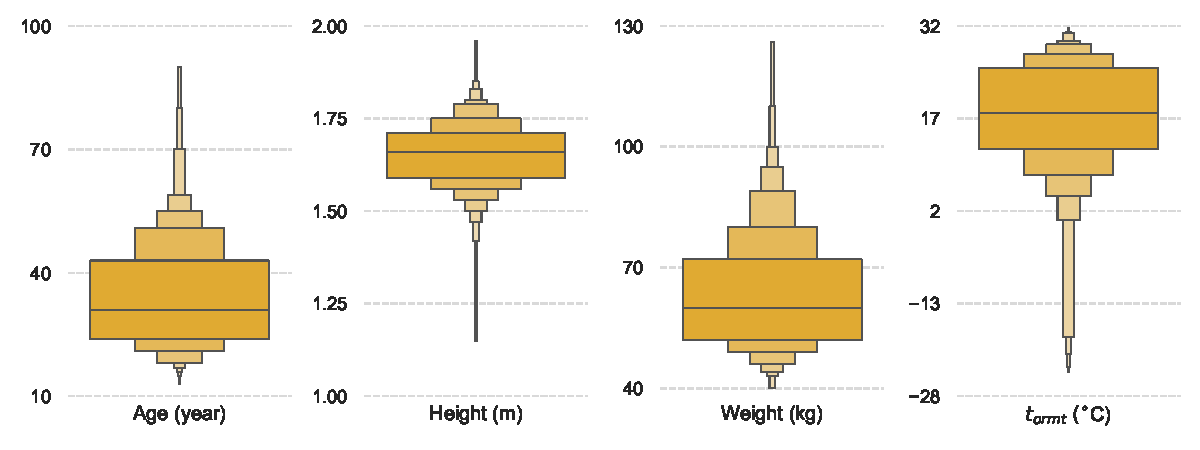
\includegraphics[width=\textwidth]{figures/dist_other_data}
    \caption{Distribution of age, height, weight, and running mean outdoor temperature.
    The data are grouped by sex.
    The text in blue is showing the the 2.5th, 50th (median), and 97.5th percentiles.}
    \label{fig:dist_other_data}
\end{figure}

The percentage of \ac{tpv} grouped by each \ac{tsv} is shown on the left side of Figure~\ref{fig:bar_plot_tp_by_ts}.
Only \var{entries_with_tp} entries had information about both \ac{tsv} and \ac{tpv}.
Thus, on the right we show a bar chart depicting the distribution of all the \ac{tsv} votes, we have used in the analysis.
The \gls{db2} in respect to the \ac{tsv} is unbalanced.
Approximately \var{perc_tsv_neutral} of all the entries have a \ac{tsv} of `Neutral'.
While less than \var{perc_tsv_hot} of the total sample of participants reported to be either `Hot' or `Cold'.

\begin{figure}[htb!]
    \centering
    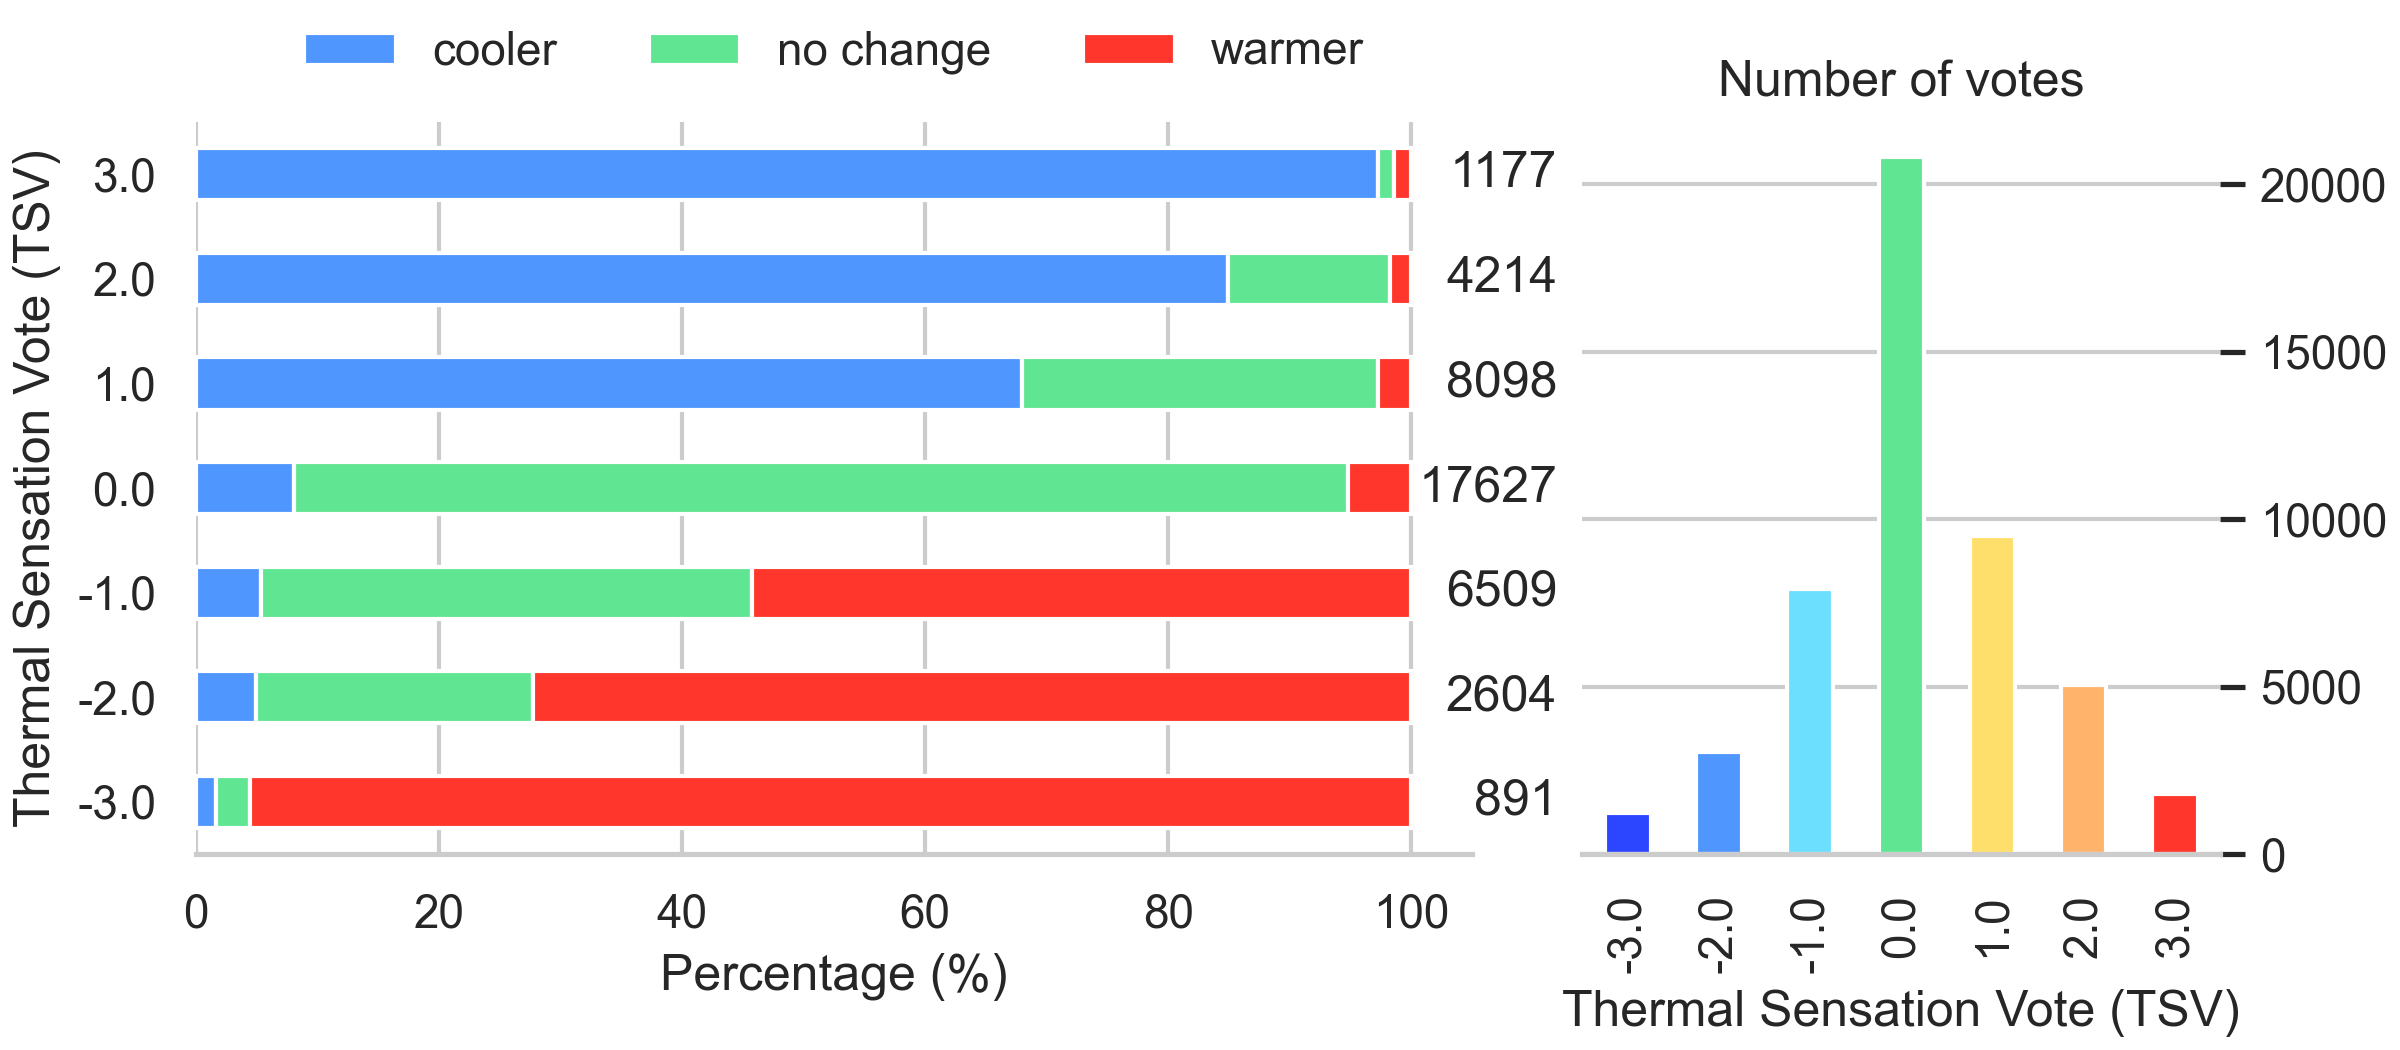
\includegraphics[width=\textwidth]{figures/bar_plot_tp_by_ts}
    \caption{The left Figure shows the percentage of \ac{tpv} for each thermal sensation vote.
    The numbers on the right side of each bar show the number of points for each \ac{tsv}.
    The right figure shows the total number of data points grouped by \ac{tsv}.
    Each bin in the Figure of the right has more data points than in the Figure on the left since information about the occupants \ac{tpv} were not always available.}
    \label{fig:bar_plot_tp_by_ts}
\end{figure}

\subsection{Comparison of PMV accuracy in predicting thermal sensation}\label{subsec:model-accuracy-comparison-in-predicting-thermal-sensation}
The \ac{pmv} was developed with the primary aim of predicting \ac{tsv}, consequently, in this Section we are reporting the prediction accuracy of different \ac{pmv} formulations.

\begin{figure}[htb!]
    \centering
    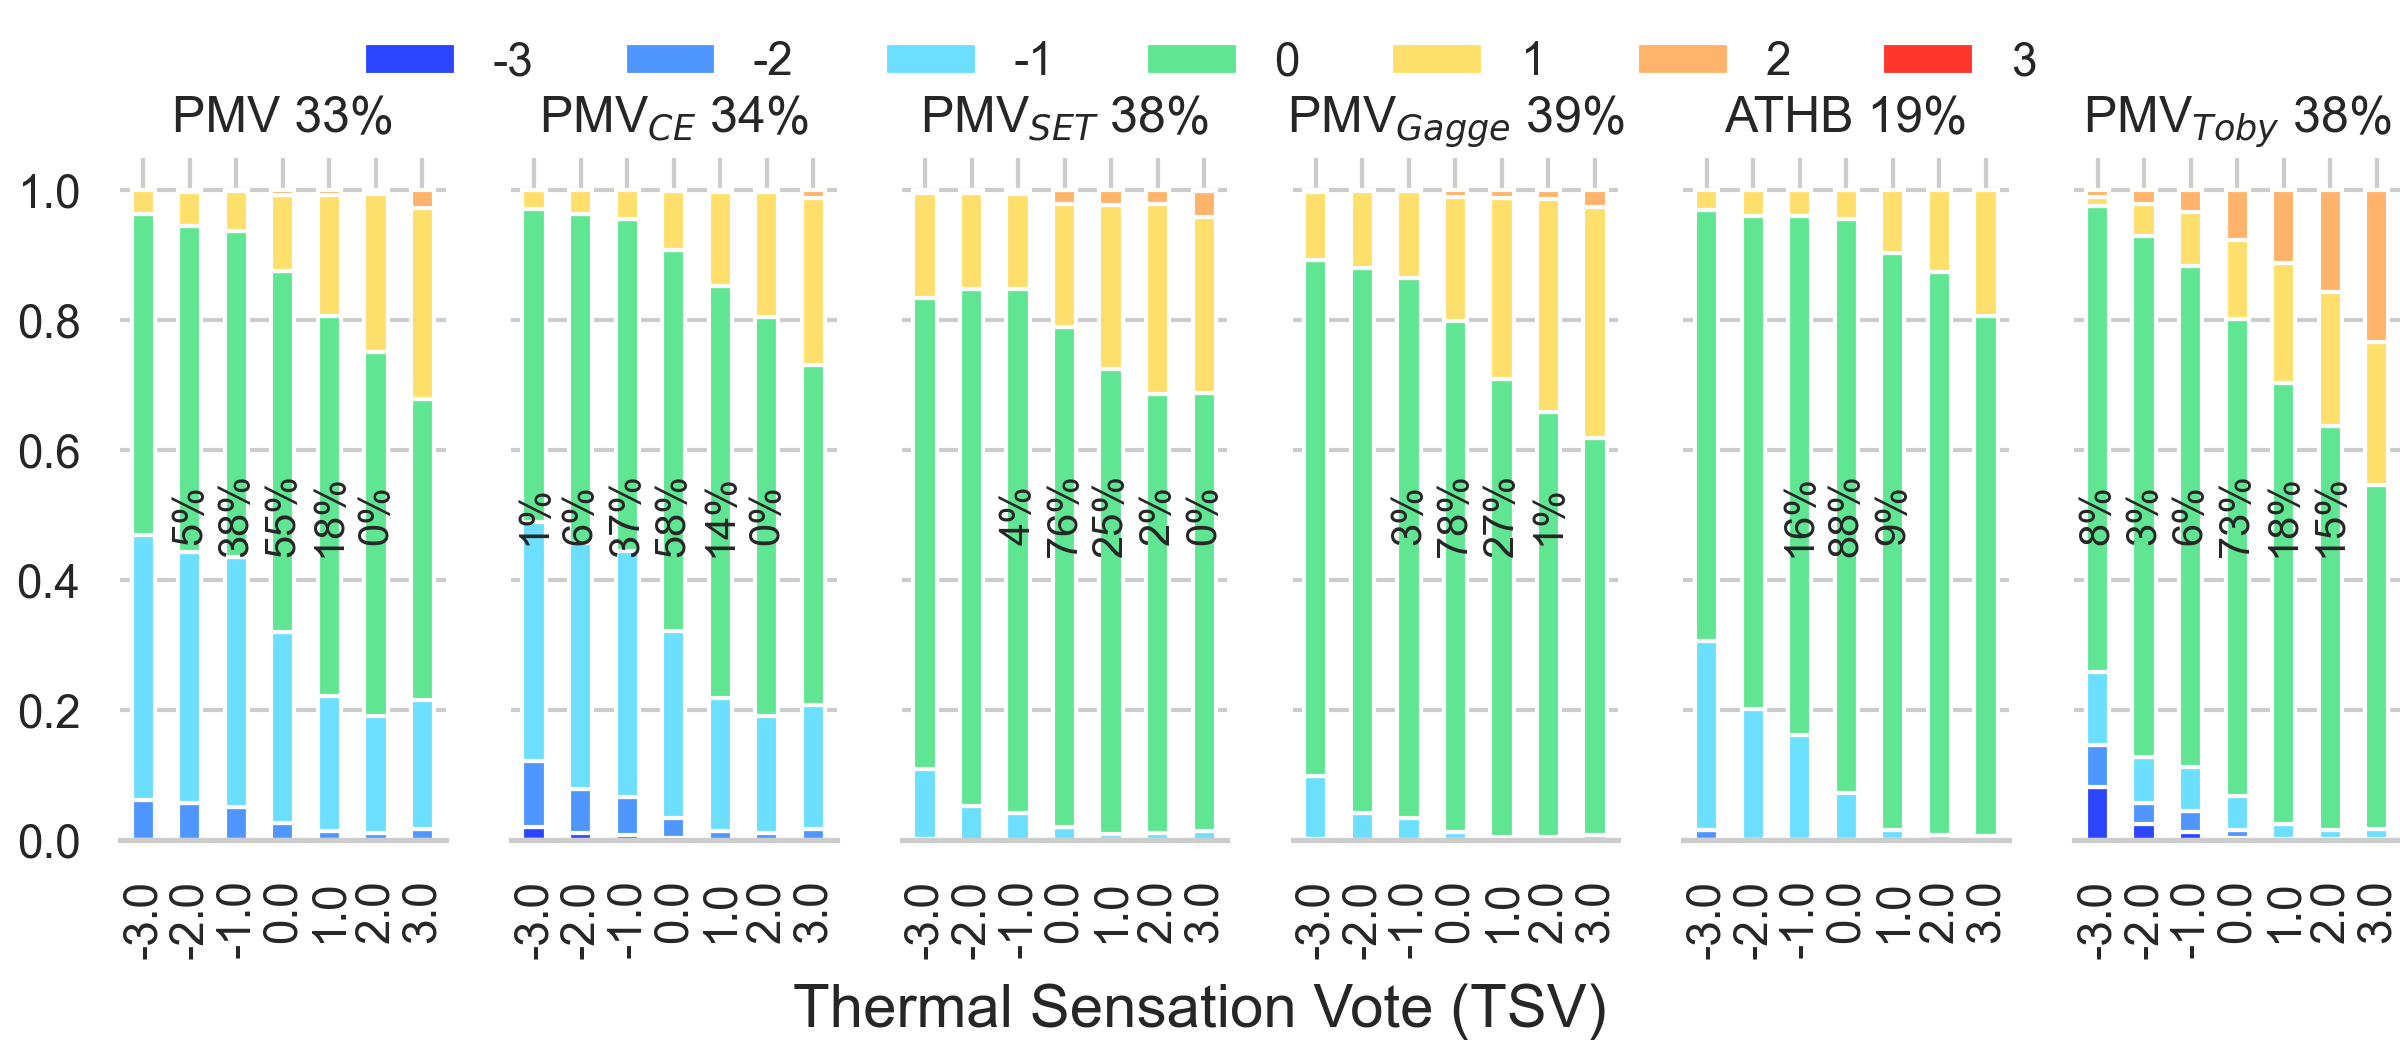
\includegraphics[width=\textwidth]{figures/bar_stacked_model_accuracy}
    \caption{}
    \label{fig:bar_stacked_model_accuracy}
\end{figure}

Being \ac{tsv} the value reported by participants (i.e., ground truth) we grouped participants responses by \ac{tsv} and reported the simple accuracy of the different \ac{pmv} formulations in Figure~\ref{fig:bar_stacked_model_accuracy}.
In other words, all \ac{pmv} formulations underestimated the conditions at which participants are thermally dissatisfied with their environment.
The overall accuracy of the \gls{pmv-ce} and \ac{pmv} were \qty{34}{\percent} and \qty{33}{\percent}, respectively.
Being the classification problem unbalanced the simple accuracy is not an optimal metric to rate the model prediction accuracy since a default strategy of guessing the majority class would lead to a high overall model accuracy.
A model that would have predicted always `neutral' would have achieved an overall accuracy of \var{perc_tsv_neutral}, which is the number of participants who voted \ac{tsv}=0.
For this reason in Table~\ref{tab:f1} we report the F1-scores for all the models.
The F1-macro score which is free from label imbalance depicts that the accuracy of both models across all metrics is marginally better to random guessing (i.e., \qty{14.3}{\percent}).

\begin{table}[htb!]
    \centering
    \begin{tabular}{lccc}
\toprule
F1 score & PMV & PMV$_{CE}$ & Dataset \\
\midrule
 micro & 0.32 & 0.34 & \multirow{3}{*}{All data} \\
macro & 0.16 & 0.15 &  \\
weighted & 0.29 & 0.30 &  \\
\specialrule{.01em}{.05em}{.05em} micro & 0.32 & 0.35 & \multirow{3}{*}{\ac{vr} $\geq$ \qty{0.2}{\m\per\s}} \\
macro & 0.17 & 0.17 &  \\
weighted & 0.30 & 0.31 &  \\
\specialrule{.01em}{.05em}{.05em} micro & 0.30 & 0.31 & \multirow{3}{*}{\ac{vr} $\geq$ \qty{0.2}{\m\per\s} at three heights} \\
macro & 0.17 & 0.16 &  \\
weighted & 0.27 & 0.27 &  \\
\specialrule{.01em}{.05em}{.05em} micro & 0.43 & 0.45 & \multirow{3}{*}{$\lvert \textrm{PMV}\lvert \leq 1.5$ and $\lvert \textrm{TSV}\lvert \leq 1.5$} \\
macro & 0.23 & 0.22 &  \\
weighted & 0.42 & 0.43 &  \\
\bottomrule
\end{tabular}
\label{tab:f1}
\end{table}

Moreover, while the \gls{pmv-ce} was specifically developed to more accurately estimate latent and sensible heat losses from the skin to the environment.
Our results show that neither formulations can correctly classify participants who reported to be either `warm' or `hot' and the \gls{pmv-ce} is less accurate than the \ac{pmv} in predicting people who were `slightly warm'.
Both models had an accuracy lower than \qty{1}{\percent} when predicting wither `warm', `hot', or `cold'.
This value is significantly lower and worse than random guessing.

Grouping the results into discrete categories introduces rounding errors since some participants reported \ac{tsv} on a continuous scale and the \ac{pmv} value is a continuous variables.
To compensate for this we plotted the \ac{pmv} values as a function of \ac{tsv} in Figure~\ref{fig:bubble_models_vs_tsv} and we plotted a lowess curve.
The curve is calculated using the individual data and not the binned data.
We binned the data only to aid the visualization of a large dataset.
If the model is to accurately predict the thermal sensation of people, the regression line should pass through the origin of the cartesian plane and a slope of 1.
As depicted in Figure~\ref{fig:bar_stacked_model_accuracy}, while the regression line does not intercept is not zero, the intercepts for the \ac{pmv} is \qty{-0.23} and for the \gls{pmv-ce} is \qty{-0.24}.

\begin{figure}[htb!]
    \centering
    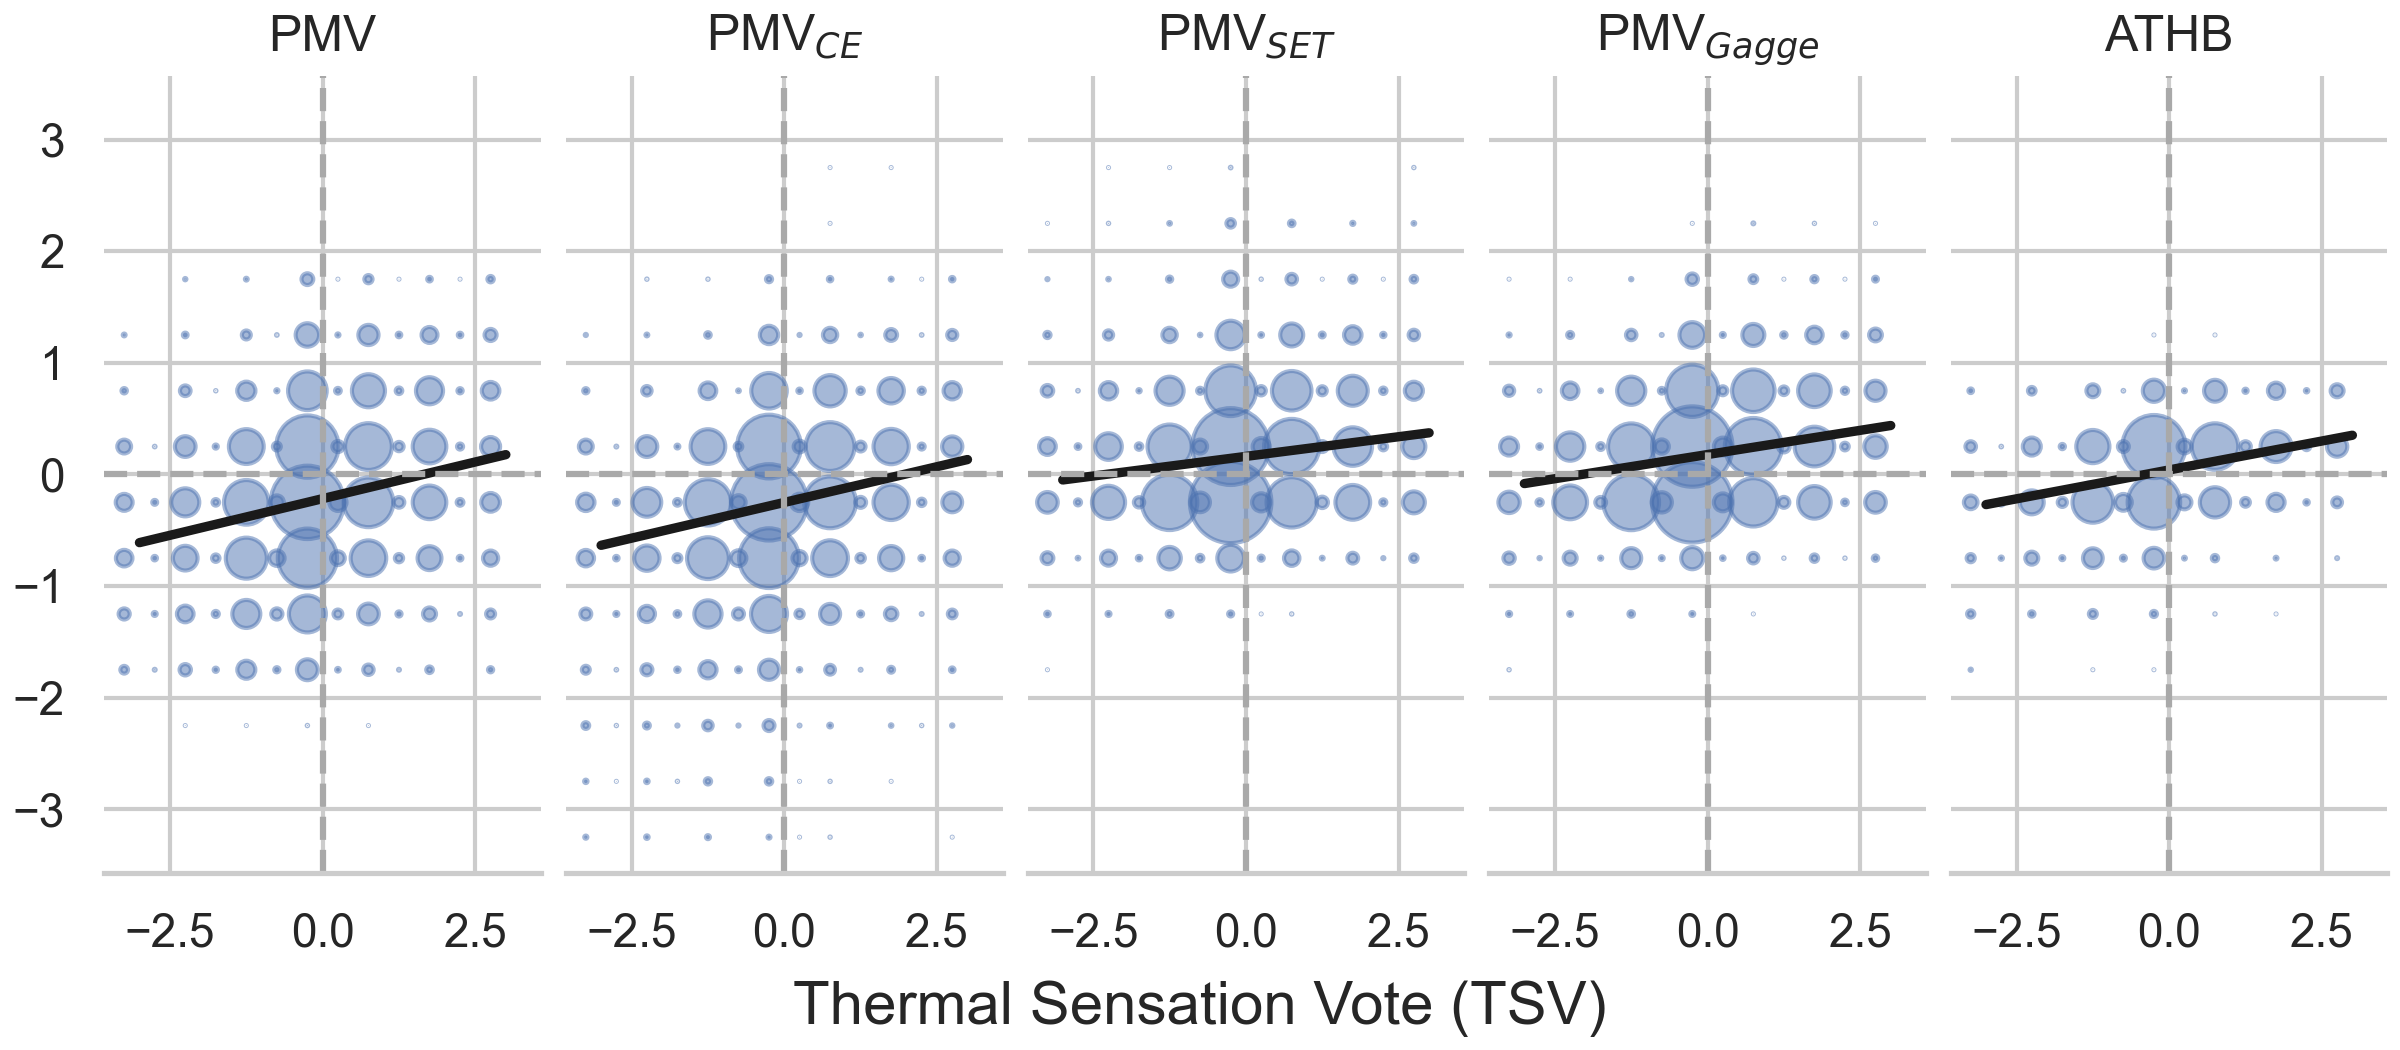
\includegraphics[width=\textwidth]{figures/bubble_models_vs_tsv}
    \caption{}
    \label{fig:bubble_models_vs_tsv}
\end{figure}

\section{Model Bias}\label{sec:model-bias}
\subsection{Model Overall Bias}\label{subsec:model-overall-bias}
As previously mentioned in the Methodology section, the aim of the \ac{pmv} model is not to accurately predict each individual thermal response form participants.
The \ac{pmv} model was developed to predict the average thermal sensation of a large group of occupants sharing the same environment.
Consequently, we calculated the overall bias of the model by subtracting the \ac{pmv} model prediction from the self-reported \ac{tsv}.
Results are presented in Figure~\ref{fig:hist_discrepancies} and show that overall the \ac{pmv} model appear to be free from serius bias.

% todo comparison models for v0.3 m/s

\begin{figure}[htb!]
    \centering
    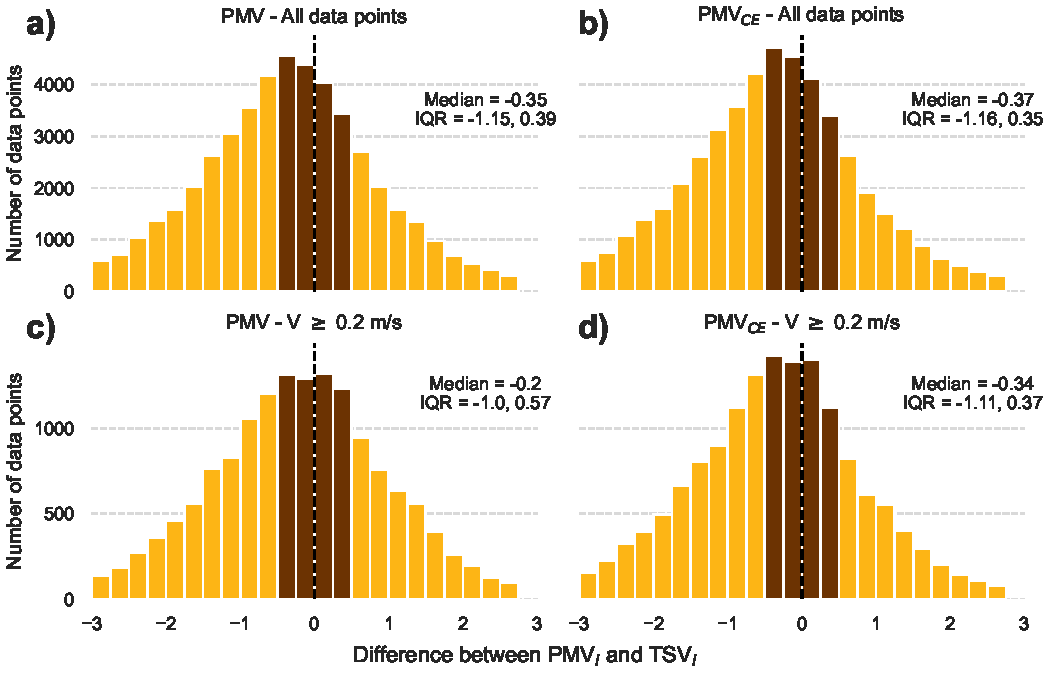
\includegraphics[width=\textwidth]{figures/hist_discrepancies}
    \caption{}
    \label{fig:hist_discrepancies}
\end{figure}

\subsection{Model Bias as Function of Independent Variables, Thermal Sensation, Thermal Preference, and PMV}\label{subsec:model-bias-variable}
To better indentify under which environmental conditions as well as how the model bias varied as a function of \ac{tsv}, \ac{tpv}, and \ac{pmv} in the Figures below we present the same results as shown in Figure~\ref{fig:hist_discrepancies} but this time we have binned the results into discrete intervals of the above-mentioned variables.
In the respective figures we are depicting the bin interval and the number of points in each bin.
We did not present the results if the number of points in the bin are lower than XXX.
% todo see if I need to implement the above

\begin{figure}[htb!]
    \centering
    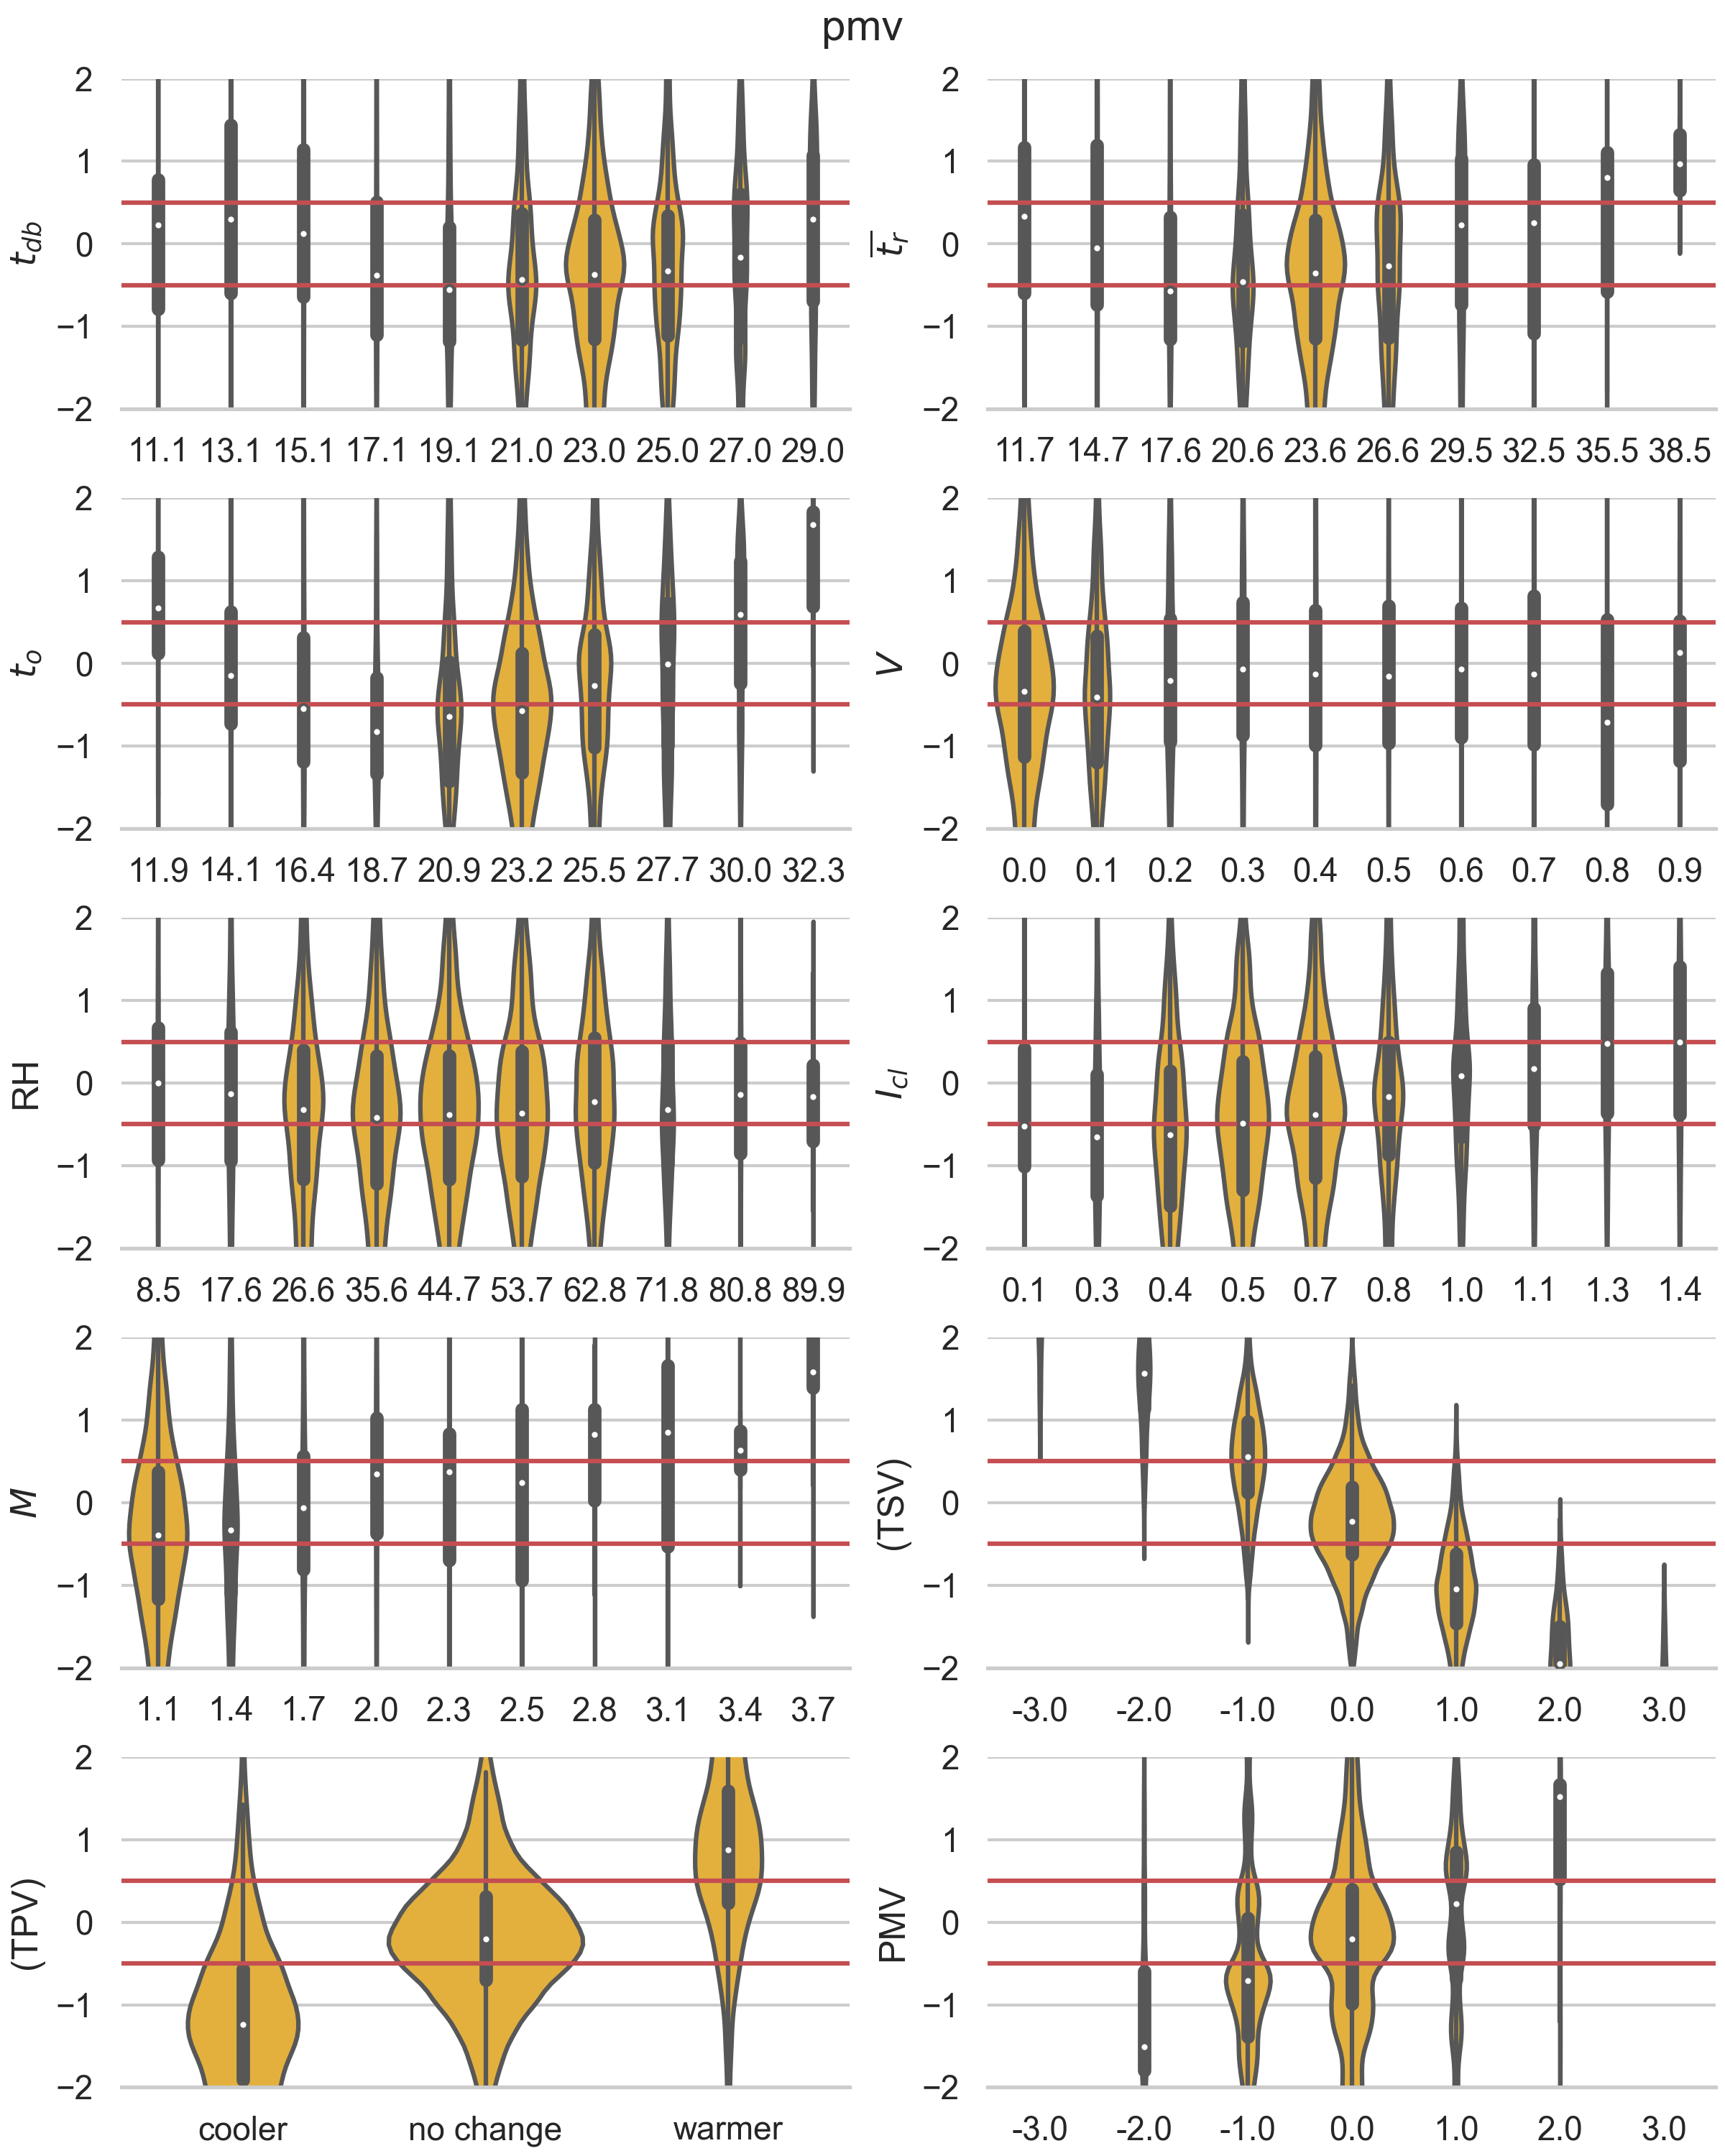
\includegraphics[width=\textwidth]{figures/bias_pmv}
    \caption{}
    \label{fig:bias_pmv}
\end{figure}

\begin{figure}[htb!]
    \centering
    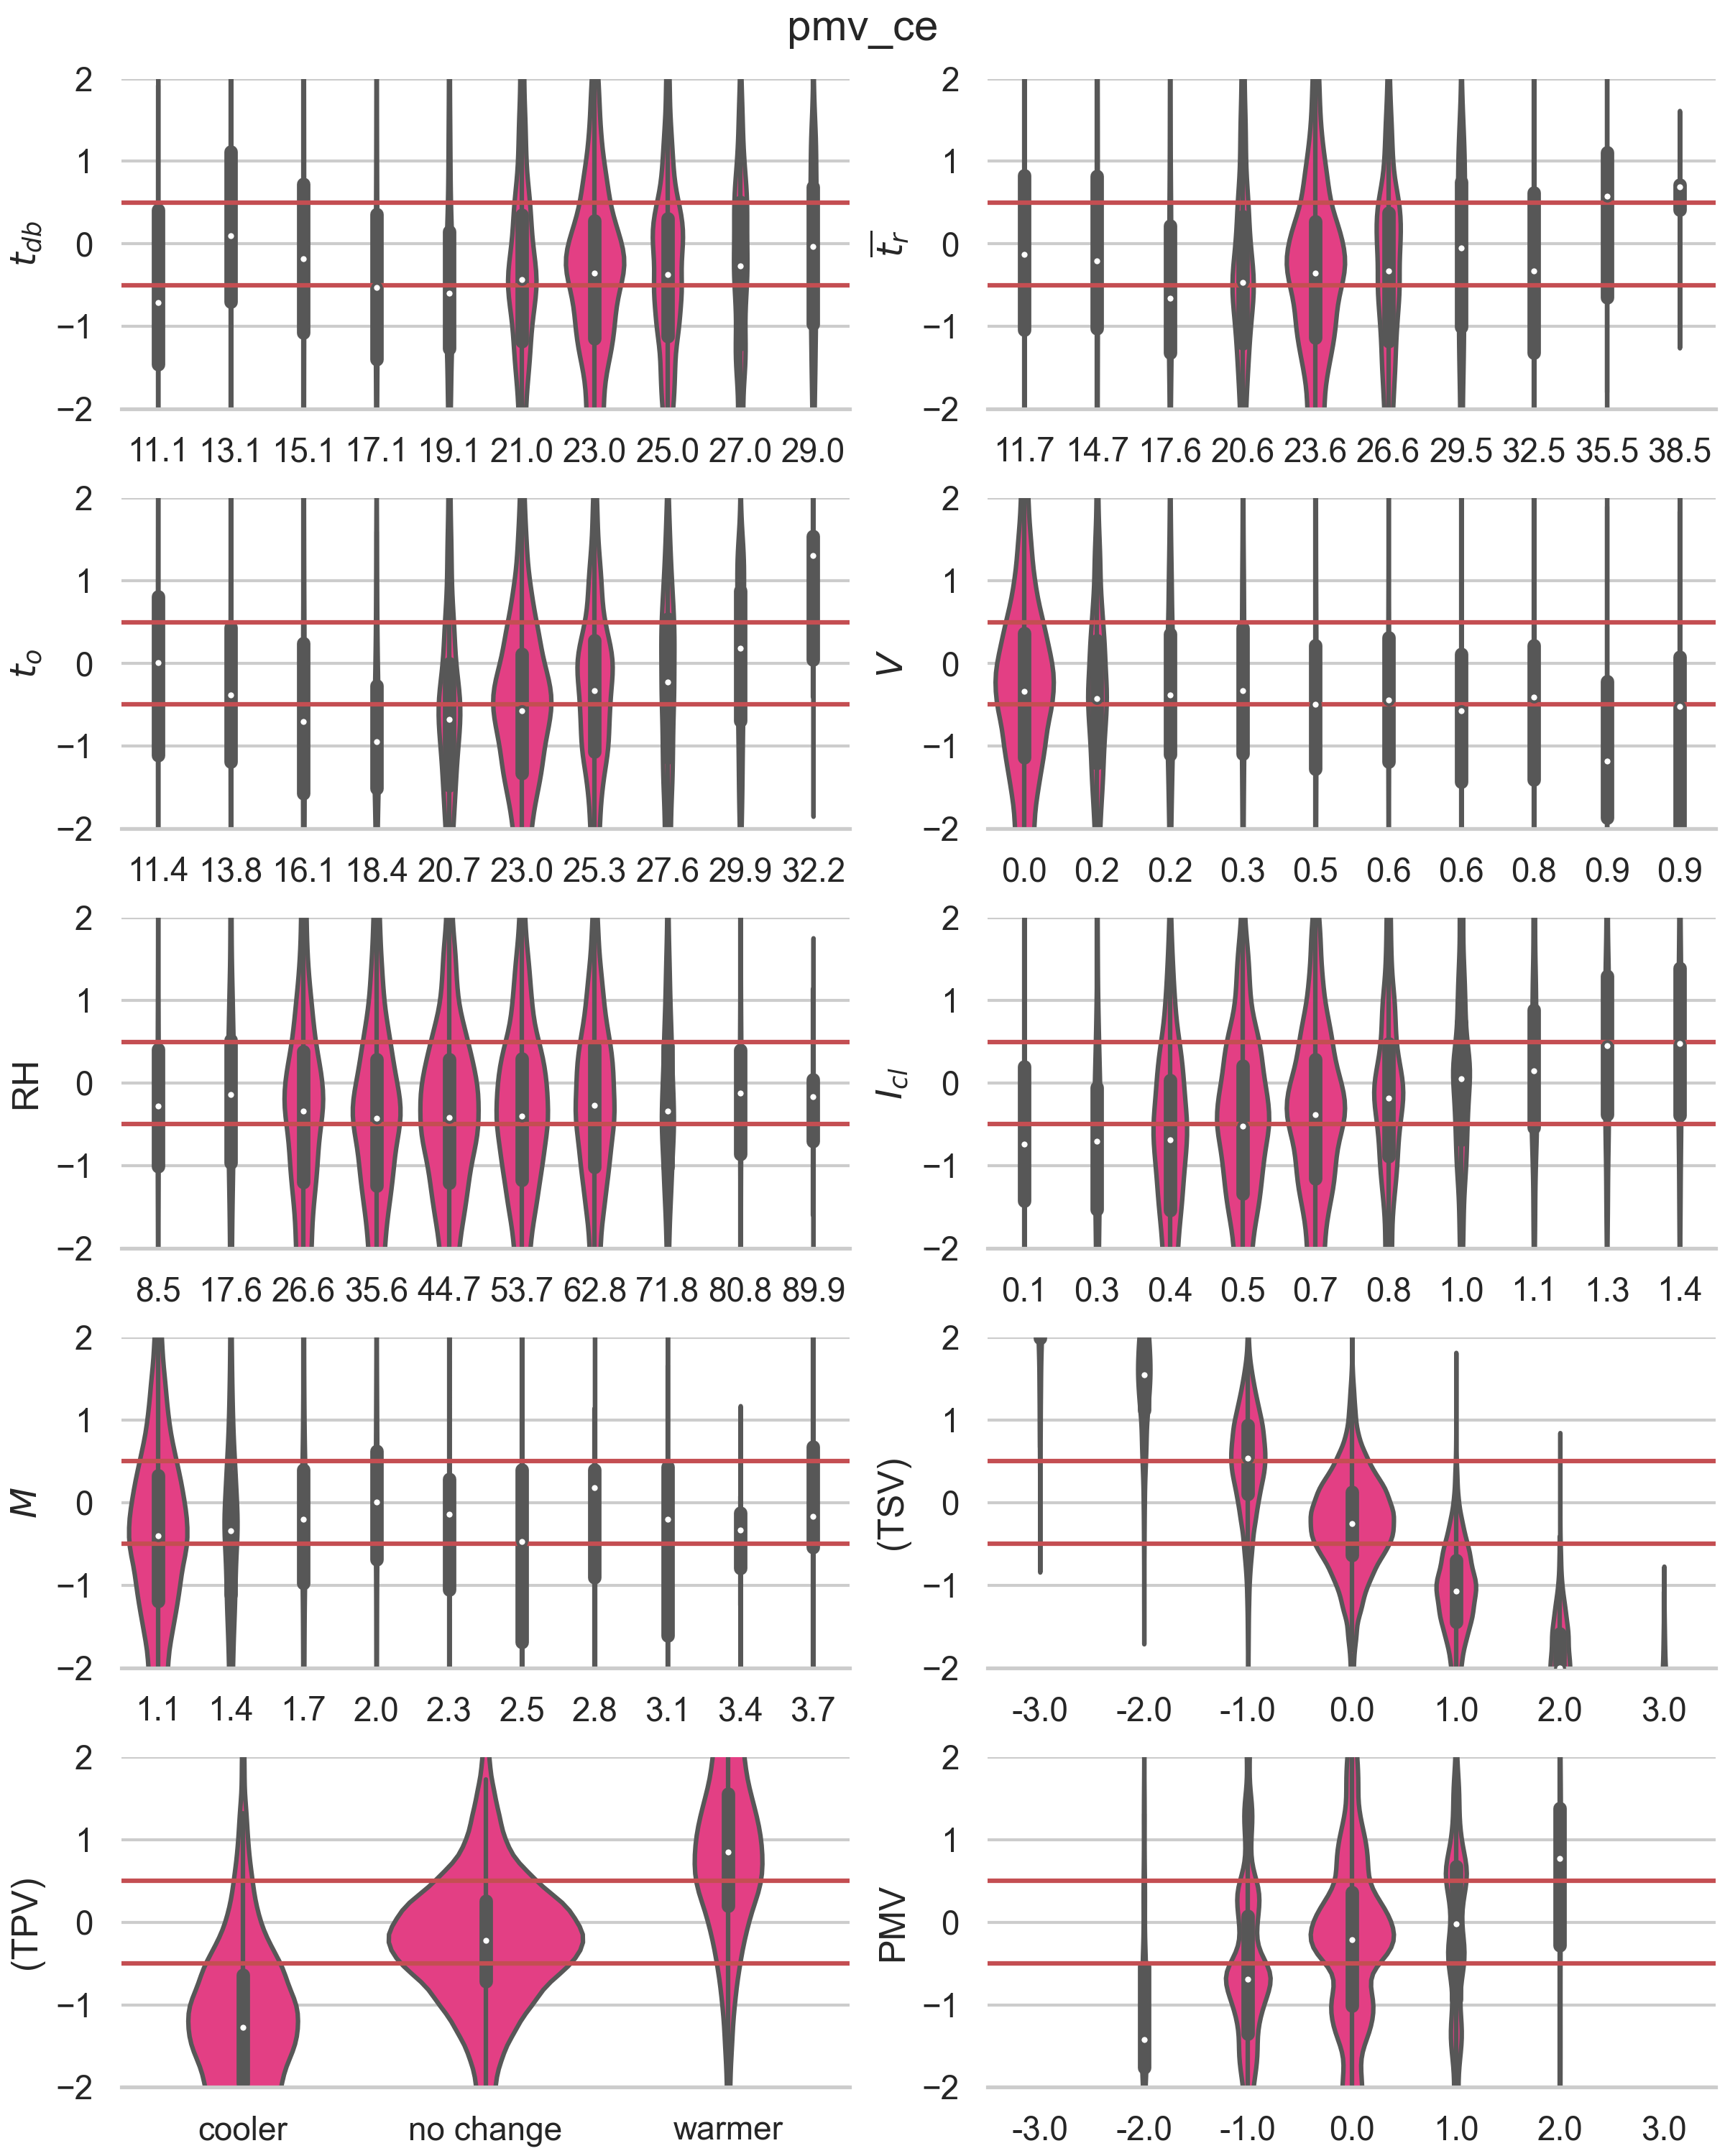
\includegraphics[width=\textwidth]{figures/bias_pmv_ce}
    \caption{}
    \label{fig:bias_pmv_ce}
\end{figure}